\chapter{Desenvolvimento do projeto}
\label{chap:metod}
Nesta seção será descrito o procedimento utilizado para construção inicial do portifólio pedido pelo cliente.
\section{Metodologia do projeto}
A metodologia utilizada para o desenvolvimento deste projeto foi baseada no modelo \textit{kanban}, que é um modelo de desenvolvimento que visa otimizar o fluxo de trabalho e a entrega de valor. Este modelo é caracterizado por um sitema visual, onde tarefas são representadas por cartões que se movem ao longo de colunas, representando o andamento do projeto. As colunas que representam as fases do modelo \textit{kanban} incluem: a fazer, em progresso, checagem, e concluido.

\section{Ideação}
  Depois da primeira reunião com o cliente e da retirada dos requisitos, já conseguimos identificar que nosso cliente é do tipo mais simples, e com base nisso decidimos criar um site/portfólio que fosse simples e prático, com isso em mente tivemos a ideia de criar um site one page com todas as informações principais do nosso cliente.

\section{Arquitetura Geral}
 A arquitetura geral, apresentada na Figura \ref{fig:arquitetura_geral}, relaciona de modo geral a interface do usuário, com a central de gerenciamento do site. Neste contexto, a interface do usuário representa o contato direto com o usuário por meio de site.
Para a central de gerenciamento do site utilizou-se o VScode. Neste cojunto se encontram as principais funcionalidades do site: mostrar as informações do cliente, navegação, atrair empregadores e empregar o cliente. Por fim, no conjunto de saídas estão os elemetos visuais.
\begin{figure} [h!]	
    \centering
    \caption{Minha arquitetura geral}
    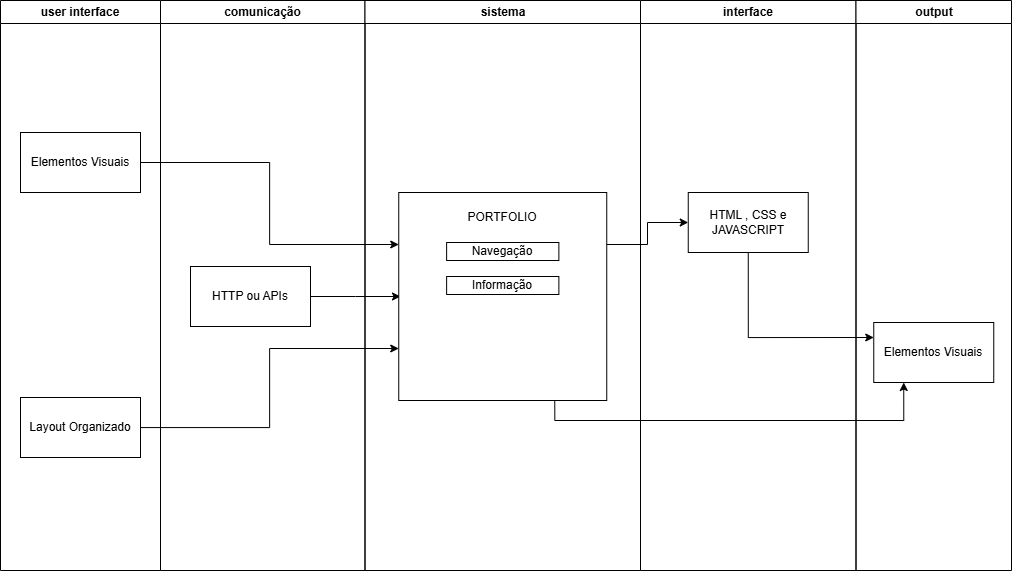
\includegraphics[width=0.8\textwidth]{Figures/arquitetura-solução.png}
    \caption*{Fonte: Autoria própria.}
    \label{fig:arquitetura_geral}
\end{figure}

\section{Requisitos técnicos}
 O portfólio foi desenvolvido em HTML e CSS, porem não contém mais requisitos tecnicos, foi um desenvolvimento mas básico.

\section{Modelagem dos processos}
 Modelagem dos processos \ref{fig:modelagem_processos} é uma técnica utilizada para representar, analisar, melhorar e automatizar os processos de uma organização. Ela descreve como as atividades são realizadas, quem as executa, quais recursos são usados e quais resultados são produzidos.
 \begin{figure} [h!]	
    \centering
    \caption{Minha modelagem de processos}
    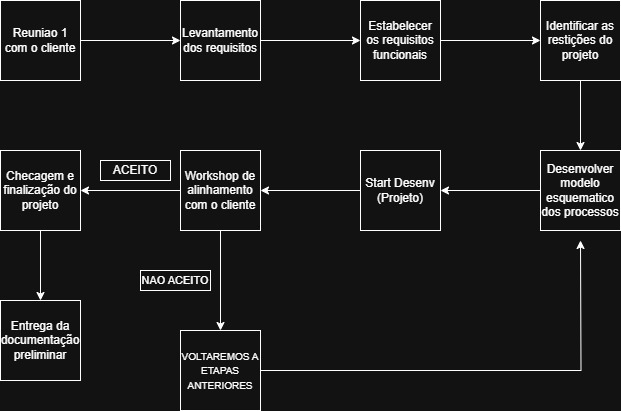
\includegraphics[width=0.8\textwidth]{Figures/modelagem_processos.jpeg}
    \caption*{Fonte: Autoria própria.}
    \label{fig:modelagem_processos}
\end{figure}